% This is text associated with the open textbook "Open Electromagnetics"
% See immediately below for author, date
% <License info goes here (boilerplate, not read by project compiler)>

%ORB TITLE Reciprocity
%ORB AUTHOR 0        # S.W. Ellingson, Virginia Tech (ellingson@vt.edu)
%ORB DATE 20191212   # yyyymmdd
%ORB ABSTRACT 

\label{m0214_Reciprocity} % <-- Must match name of this file and module directory name.  Don't mess with this!
\index{reciprocity|(}

The term ``reciprocity'' refers to a class of theorems that relate the inputs and outputs of a linear system to those of an identical system in which the inputs and outputs are swapped.  
The importance of reciprocity in electromagnetics is that it simplifies problems that would otherwise be relatively difficult to solve.  
An example of this is the derivation of the receiving properties of antennas, which is addressed in other sections using results derived in this section.

As an initial and relatively gentle introduction, consider a well-known special case that emerges in basic circuit theory: The two-port device shown in Figure~\ref{m0214_fTwoPort}.
%
\begin{figure}[b!] % <--- "[b!]" for first figure in section *only*; delete for 2nd and subsequent figures
\begin{center}
\pdftooltip{{  % note double braces
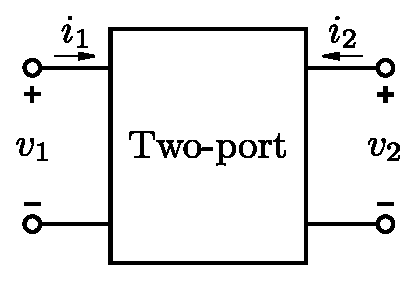
\includegraphics[width=1.5in]{modules/m0214_fTwoPort.eps} 
% https://commons.wikimedia.org/wiki/File:Two_Port_Circuit.svg
}}{Rectangle labeled Two-port with 2 open terminals facing left and right. Left terminal small v subscript 1 and right terminal small v subscript 2 with upper limit positive. Current small i subscript 1 (left) and small i subscript 2 (right), both enter the device from the positive terminal.}
\end{center}
\centerline{\scriptsize 
\hyperref[m0214_fTwoPort_Credit]{Inductiveload}, 
public domain
(modified) 
} % \centerline 
\caption{
\label{m0214_fTwoPort}
Two-port device.
}
\end{figure}
%
The two-port is said to be reciprocal if the voltage $v_2$ appearing at port~2 due to a current applied at port~1 is the same as $v_1$ when the same current is applied instead at port~2. 
This is normally the case when the two-port consists exclusively of linear passive devices such as ideal resistors, capacitors, and inductors.
The fundamental underlying requirement is linearity: That is, outputs must be proportional to inputs, and superposition must apply.  

This result from basic circuit theory is actually a special case of a more general theorem of electromagnetics, which we shall now derive.
Figure~\ref{m0214_fReciprocity1} shows a scenario in which a current distribution $\widetilde{\bf J}_1$ is completely contained within a volume $\mathcal{V}$. 
%
\begin{figure} % <--- "[b!]" for first figure in section *only*; delete for 2nd and subsequent figures
\begin{center}
\pdftooltip{{  % note double braces

\includegraphics[width=1.5in]{modules/m0214_fReciprocity1.eps} 
% https://commons.wikimedia.org/wiki/File:An_electromagnetic_system_consisting_of_a_current_distribution_radiating_an_electric_field.svg
}}{Dashed rounded rectangle contains a dashed circle. Inside the circle 3 arrows all pointing northwest and labeled capital J tilde subscript 1. The rectangle region labeled capital V (bottom right), capital E tilde subscript 1 (upper right), and the group epsilon, mu, sigma (bottom left).}
\end{center}
\centerline{\scriptsize 
\copyright~\hyperref[m0214_fReciprocity1_Credit]{C.\ Wang} 
\href{https://creativecommons.org/licenses/by-sa/4.0/}{CC BY-SA 4.0} 
} % \centerline 
\caption{
\label{m0214_fReciprocity1}
An electromagnetic system consisting of a current distribution $\widetilde{\bf J}_1$ radiating an electric field $\widetilde{\bf E}_1$ in the presence of linear matter.
}
\end{figure}
%
\begin{figure} % <--- "[b!]" for first figure in section *only*; delete for 2nd and subsequent figures
\begin{center}
\pdftooltip{{  % note double braces
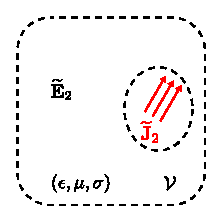
\includegraphics[width=1.5in]{modules/m0214_fReciprocity2.eps} 
% https://commons.wikimedia.org/wiki/File:An_electromagnetic_system_consisting_of_a_different_current_distribution_radiating_an_electric_field.svg
}}{Dashed rounded rectangle contains a dashed circle. Inside the circle 3 arrows all pointing northeast and labeled capital J tilde subscript 2. The rectangle region labeled capital V (bottom right), capital E tilde subscript 2 (upper right), and the group epsilon, mu, sigma (bottom left).}
\end{center}
\centerline{\scriptsize 
\copyright~\hyperref[m0214_fReciprocity2_Credit]{C.\ Wang} 
\href{https://creativecommons.org/licenses/by-sa/4.0/}{CC BY-SA 4.0} 
} % \centerline  
\caption{
\label{m0214_fReciprocity2}
The same electromagnetic system as shown in Figure~\ref{m0214_fReciprocity1} (including the same distribution of matter), but now with a different input, $\widetilde{\bf J}_2$, resulting in a different output, $\widetilde{\bf E}_2$.
}
\end{figure}
%
This current is expressed as a volume current density, having SI base units of A/m$^2$.  Also, the current is expressed in phasor form, signaling that we are considering a single frequency.  This current distribution gives rise to an electric field intensity $\widetilde{\bf E}_1$, having SI base units of V/m.  
The volume may consist of any combination of linear time-invariant matter; i.e., permittivity $\epsilon$, permeability $\mu$, and conductivity $\sigma$ are constants that may vary arbitrarily with position but not with time.

Here's a key idea:  We may interpret this scenario as a ``two-port'' system in which 
$\widetilde{\bf J}_1$ is the input, $\widetilde{\bf E}_1$ is the output, and the system's behavior is completely defined by Maxwell's equations in differential phasor form:
\index{Maxwell's equations!differential phasor form}
%
\begin{equation}
\nabla \times  \widetilde{\bf E}_1 = -j\omega\mu\widetilde{\bf H}_1 
\label{m0214_eMCE1}
\end{equation}
%
\begin{equation}
\nabla \times \widetilde{\bf H}_1  = \widetilde{\bf J}_1 + j\omega\epsilon\widetilde{\bf E}_1
\label{m0214_eMCH1} 
\end{equation}
% 
along with the appropriate electromagnetic boundary conditions.
\index{boundary conditions}
(For the purposes of our present analysis, $\widetilde{\bf H}_1$ is neither an input nor an output; it is merely a coupled quantity that appears in this particular formulation of the relationship between $\widetilde{\bf E}_1$ and $\widetilde{\bf J}_1$.)

Figure~\ref{m0214_fReciprocity2} shows a scenario in which a different current distribution $\widetilde{\bf J}_2$ is completely contained within the same volume $\mathcal{V}$ containing the same distribution of linear matter. 
This new current distribution gives rise to an electric field intensity $\widetilde{\bf E}_2$.  
The relationship between $\widetilde{\bf E}_2$ and $\widetilde{\bf J}_2$ is governed by the same equations:
%
\begin{equation}
\nabla \times  \widetilde{\bf E}_2 = -j\omega\mu\widetilde{\bf H}_2 
\label{m0214_eMCE2}
\end{equation}
%
\begin{equation}
\nabla \times \widetilde{\bf H}_2  = \widetilde{\bf J}_2 + j\omega\epsilon\widetilde{\bf E}_2
\label{m0214_eMCH2} 
\end{equation}
%
along with the same electromagnetic boundary conditions.
Thus, we may interpret this scenario as the \emph{same} electromagnetic system depicted in Figure~\ref{m0214_fReciprocity1}, except now with 
$\widetilde{\bf J}_2$ as the input and $\widetilde{\bf E}_2$ is the output. 

The input current and output field in the second scenario are, in general, completely different from the input current and output field in the first scenario.  However, both scenarios involve precisely the same electromagnetic system; i.e., the same governing equations and the same distribution of matter.
This leads to the following question:
Let's say you know nothing about the system, aside from the fact that it is linear and time-invariant.
However, you are able to observe the first scenario; i.e., you know $\widetilde{\bf E}_1$ in response to $\widetilde{\bf J}_1$.
Given this very limited look into the behavior of the system, what can you infer about $\widetilde{\bf E}_2$ given $\widetilde{\bf J}_2$, or vice-versa?
At first glance, the answer might seem to be nothing, since you lack a description of the system.
However, the answer turns out to be that a surprising bit more information is available.
This information is provided by reciprocity.
To show this, we must engage in some pure mathematics.  

{\bf Derivation of the Lorentz reciprocity theorem.}
\index{Lorentz reciprocity theorem|(}
First, let us take the dot product of $\widetilde{\bf H}_2$ with each side of Equation~\ref{m0214_eMCE1}:
%
\begin{equation}
\widetilde{\bf H}_2 \cdot \left( \nabla \times  \widetilde{\bf E}_1 \right) = -j\omega\mu\widetilde{\bf H}_1 \cdot \widetilde{\bf H}_2 
\label{m0214_e5}
\end{equation}
%
Similarly, let us take the dot product of $\widetilde{\bf E}_1$ with each side of Equation~\ref{m0214_eMCH2}:
%
\begin{equation}
\widetilde{\bf E}_1 \cdot \left( \nabla \times  \widetilde{\bf H}_2 \right) = \widetilde{\bf E}_1 \cdot \widetilde{\bf J}_2 +j\omega\epsilon\widetilde{\bf E}_1 \cdot \widetilde{\bf E}_2 
\label{m0214_e6}
\end{equation}
%
Next, let us subtract Equation~\ref{m0214_e5} from Equation~\ref{m0214_e6}.  
The left side of the resulting equation is 
%
\begin{equation}
\widetilde{\bf E}_1 \cdot \left( \nabla \times  \widetilde{\bf H}_2 \right) - \widetilde{\bf H}_2 \cdot \left( \nabla \times  \widetilde{\bf E}_1 \right)
\end{equation}
%
This can be simplified using the vector identity (Appendix~\ref{m0140_Vector_Identities}):
%
\begin{equation}
\nabla \cdot \left({\bf A}\times {\bf B}\right) = {\bf B}\cdot\left(\nabla \times{\bf A}\right)-{\bf A}\cdot\left(\nabla \times{\bf B}\right) 
\end{equation}
%
Yielding
%
\begin{equation}
\widetilde{\bf E}_1 \cdot \left( \nabla \times  \widetilde{\bf H}_2 \right) - \widetilde{\bf H}_2 \cdot \left( \nabla \times  \widetilde{\bf E}_1 \right) = \nabla \cdot \left(\widetilde{\bf H}_2 \times \widetilde{\bf E}_1 \right)
\end{equation}
%
So, by subtracting Equation~\ref{m0214_e5} from Equation~\ref{m0214_e6}, we have found:
%
\begin{equation}
\nabla \cdot \left(\widetilde{\bf H}_2 \times \widetilde{\bf E}_1 \right)
= \widetilde{\bf E}_1 \cdot \widetilde{\bf J}_2 
+j\omega\epsilon\widetilde{\bf E}_1 \cdot \widetilde{\bf E}_2 
+j\omega\mu     \widetilde{\bf H}_1 \cdot \widetilde{\bf H}_2
\label{m0214_e7}
\end{equation}
 
Next, we repeat the process represented by Equations~\ref{m0214_e5}--\ref{m0214_e7} above to generate a complementary equation to Equation~\ref{m0214_e7}.
This time we take the dot product of $\widetilde{\bf E}_2$ with each side of Equation~\ref{m0214_eMCH1}:
%
\begin{equation}
\widetilde{\bf E}_2 \cdot \left( \nabla \times  \widetilde{\bf H}_1 \right) = \widetilde{\bf E}_2 \cdot \widetilde{\bf J}_1 +j\omega\epsilon\widetilde{\bf E}_1 \cdot \widetilde{\bf E}_2 
\label{m0214_e8}
\end{equation}
%
Similarly, let us take the dot product of $\widetilde{\bf H}_1$ with each side of Equation~\ref{m0214_eMCE2}:

\begin{equation}
\widetilde{\bf H}_1 \cdot \left( \nabla \times  \widetilde{\bf E}_2 \right) = -j\omega\mu\widetilde{\bf H}_1 \cdot \widetilde{\bf H}_2 
\label{m0214_e9}
\end{equation}
%
Next, let us subtract Equation~\ref{m0214_e9} from Equation~\ref{m0214_e8}. 
Again using the vector identity, the left side of the resulting equation is 
%
\begin{equation}
\widetilde{\bf E}_2 \cdot \left( \nabla \times  \widetilde{\bf H}_1 \right) - \widetilde{\bf H}_1 \cdot \left( \nabla \times  \widetilde{\bf E}_2 \right) = \nabla \cdot \left(\widetilde{\bf H}_1 \times \widetilde{\bf E}_2 \right)
\end{equation}
%
So we find:
%
\begin{equation}
\nabla \cdot \left(\widetilde{\bf H}_1 \times \widetilde{\bf E}_2 \right)
= \widetilde{\bf E}_2 \cdot \widetilde{\bf J}_1 
+j\omega\epsilon\widetilde{\bf E}_1 \cdot \widetilde{\bf E}_2 
+j\omega\mu     \widetilde{\bf H}_1 \cdot \widetilde{\bf H}_2
\label{m0214_e10}
\end{equation}

Finally, subtracting Equation~\ref{m0214_e10} from Equation~\ref{m0214_e7}, we obtain:
%
\begin{equation}
\nabla \cdot \left(\widetilde{\bf H}_2 \times \widetilde{\bf E}_1 - \widetilde{\bf H}_1 \times \widetilde{\bf E}_2 \right)
= \widetilde{\bf E}_1 \cdot \widetilde{\bf J}_2 
- \widetilde{\bf E}_2 \cdot \widetilde{\bf J}_1 
\label{m0214_eLRTD}
\end{equation}
%
This equation is commonly known by the name of the theorem it represents: The \emph{Lorentz reciprocity theorem}.
The theorem is a very general statement about the relationship between fields and currents at each point in space.
An associated form of the theorem applies to contiguous regions of space.
To obtain this form, we simply integrate both sides of Equation~\ref{m0214_eLRTD} over the volume $\mathcal{V}$:
%
\begin{flalign}
\int_{\mathcal V} {\nabla \cdot \left(\widetilde{\bf H}_2 \times \widetilde{\bf E}_1 - \widetilde{\bf H}_1 \times \widetilde{\bf E}_2 \right) } dv \nonumber \\
= 
\int_{\mathcal V} {\left( \widetilde{\bf E}_1 \cdot \widetilde{\bf J}_2 
- \widetilde{\bf E}_2 \cdot \widetilde{\bf J}_1 \right)} dv
\end{flalign}
%
We now take the additional step of using the divergence theorem (Appendix~\ref{m0140_Vector_Identities}) to transform the left side of the equation into a surface integral:
%
\begin{flalign}
\oint_{\mathcal S} {\left(\widetilde{\bf H}_2 \times \widetilde{\bf E}_1 - \widetilde{\bf H}_1 \times \widetilde{\bf E}_2 \right) \cdot d{\bf s}} \nonumber \\
= 
\int_{\mathcal V} {\left( \widetilde{\bf E}_1 \cdot \widetilde{\bf J}_2 
- \widetilde{\bf E}_2 \cdot \widetilde{\bf J}_1 \right)} dv
\label{m0214_eLRTI}
\end{flalign}
%
where $\mathcal{S}$ is the closed mathematical surface which bounds $\mathcal{V}$.
This is also the Lorentz reciprocity theorem, but now in integral form.
This version of the theorem relates fields on the bounding surface to sources within the volume.

The integral form of the theorem has a particularly useful feature.
Let us confine the sources to a finite region of space, while allowing $\mathcal{V}$ to grow infinitely large, expanding to include all space.
In this situation, the closest distance between any point containing non-zero source current and $\mathcal{S}$ is infinite.
Because field magnitude diminishes with distance from the source, the fields $(\widetilde{\bf E}_1,\widetilde{\bf H}_1)$ and $(\widetilde{\bf E}_2,\widetilde{\bf H}_2)$ are all effectively zero on $\mathcal{S}$.
In this case, the left side of Equation~\ref{m0214_eLRTI} is zero, and we find:
%
\begin{equation}
\boxed{
\int_{\mathcal V} {\left( \widetilde{\bf E}_1 \cdot \widetilde{\bf J}_2 
- \widetilde{\bf E}_2 \cdot \widetilde{\bf J}_1 \right)} dv = 0 
}
\label{m0214_eLRTI2}
\end{equation}
%
for any volume $\mathcal{V}$ which contains \emph{all} the current. 
%
%%%%%%%%%%%%%%%%%%%%%%%%%%%%%%%%%%%%%%%%%%%%%%%
%ORB HIGHLIGHT
\begin{mdframed}[backgroundcolor=yellow!20,nobreak=true] 
The \emph{Lorentz reciprocity theorem} (Equation~\ref{m0214_eLRTI2}) describes a relationship between one distribution of current and the resulting fields, and a second distribution of current and resulting fields, when both scenarios take place in identical regions of space filled with identical distributions of linear matter.
\end{mdframed}
%%%%%%%%%%%%%%%%%%%%%%%%%%%%%%%%%%%%%%%%%%%%%%%
%
%As promised earlier, we have identified something about the second scenario that was not apparent from the first scenario, and we did it without any information about the system itself.

Why do we refer to this relationship as reciprocity?
Simply because the expression is identical when the subscripts ``1'' and ``2'' are swapped.
In other words, the relationship does not recognize a distinction between ``inputs'' and ``outputs;'' there are only ``ports.''

A useful special case pertains to scenarios in which the current distributions $\widetilde{\bf J}_1$ and $\widetilde{\bf J}_2$ are \emph{spatially disjoint}.  By ``spatially disjoint,'' we mean that there is no point in space at which both $\widetilde{\bf J}_1$ and $\widetilde{\bf J}_2$ are non-zero; in other words, these distributions do not overlap.
(Note that the currents shown in Figures~\ref{m0214_fReciprocity1} and \ref{m0214_fReciprocity2} are depicted as spatially disjoint.)
To see what happens in this case, let us first rewrite Equation~\ref{m0214_eLRTI2} as follows:
%
\begin{equation}
\int_{\mathcal V} { \widetilde{\bf E}_1 \cdot \widetilde{\bf J}_2 ~dv } 
=
\int_{\mathcal V} { \widetilde{\bf E}_2 \cdot \widetilde{\bf J}_1 ~dv } 
\label{m0214_eLRTI3}
\end{equation}
%
Let $\mathcal{V}_1$ be the contiguous volume over which $\widetilde{\bf J}_1$ is non-zero, and 
let $\mathcal{V}_2$ be the contiguous volume over which $\widetilde{\bf J}_2$ is non-zero.
Then Equation~\ref{m0214_eLRTI3} may be written as follows:
%
\begin{equation}
\int_{{\mathcal V}_2} { \widetilde{\bf E}_1 \cdot \widetilde{\bf J}_2 ~dv } 
=
\int_{{\mathcal V}_1} { \widetilde{\bf E}_2 \cdot \widetilde{\bf J}_1 ~dv } 
\label{m0214_eLRTI4}
\end{equation}
%
The utility of this form is that we have reduced the region of integration to just those regions where the current exists.
\index{Lorentz reciprocity theorem|)}

{\bf Reciprocity of two-ports consisting of antennas.}
Equation~\ref{m0214_eLRTI4} allows us to establish the reciprocity of two-ports consisting of pairs of antennas.
This is most easily demonstrated for pairs of thin dipole antennas, as shown in Figure~\ref{m0214_fAnt2Port}.
%
\begin{figure} % <--- "[b!]" for first figure in section *only*; delete for 2nd and subsequent figures
\begin{center}
\pdftooltip{{  % note double braces
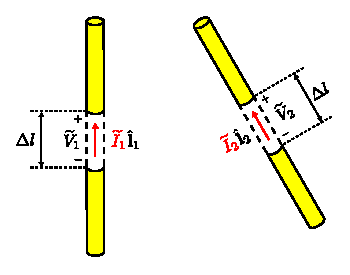
\includegraphics[width=2.5in]{modules/m0214_fAnt2Port.eps} 
% https://commons.wikimedia.org/wiki/File:A_two-port_consisting_of_two_dipole_antennas.svg
}}{Two wires, one vertical (on left) and one diagonal angled left (on right). Both wires are open in the middle a length capital delta small l. In the vertical wire, capital v tilde subscript 1 and current capital i tilde subscript 1 times capital i hat subscript 1. In the tilted wire, capital v tilde subscript 2 and current capital i tilde subscript 2 times capital i hat subscript 2.
}
\end{center}
\centerline{\scriptsize 
\copyright~\hyperref[m0214_fAnt2Port_Credit]{C.\ Wang} 
\href{https://creativecommons.org/licenses/by-sa/4.0/}{CC BY-SA 4.0} 
} % \centerline  
\caption{
\label{m0214_fAnt2Port}
A two-port consisting of two dipole antennas.
}
\end{figure}
%
Here, port~1 is defined by the terminal quantities $(\widetilde{V}_1,\widetilde{I}_1)$ of the antenna on the left, and
port~2 is defined by the terminal quantities $(\widetilde{V}_2,\widetilde{I}_2)$ of the antenna on the right.
These quantities are defined with respect to a small gap of length $\Delta l$ between the perfectly-conducting arms of the dipole. 
Either antenna may transmit or receive, so $(\widetilde{V}_1,\widetilde{I}_1)$ depends on $(\widetilde{V}_2,\widetilde{I}_2)$, and vice-versa.

The transmit and receive cases for port~1 are illustrated in Figure~\ref{m0214_fAnt1}(a) and (b), respectively.
%
\begin{figure} % <--- "[b!]" for first figure in section *only*; delete for 2nd and subsequent figures
\begin{center}
\pdftooltip{{  % note double braces
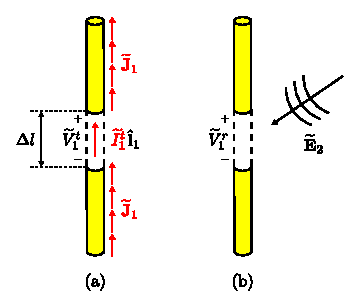
\includegraphics[width=2.5in]{modules/m0214_fAnt1.eps} 
% https://en.wikipedia.org/wiki/File:Sidelobes_en.svg
}}{Two wires. Both wires are open in the middle a length capital delta small l. In the left wire, capital v tilde subscript 1 superscript t and current capital i tilde subscript 1 superscript 1 times capital i hat subscript 1. Upward arrows run the length of the wire are labeled capital J tilde subscript 1. In the right wire, capital v tilde subscript 1 superscript 2 is approached by an angled wave labeled capital E tilde subscript 2.}
\end{center}
\centerline{\scriptsize 
\copyright~\hyperref[m0214_fAnt1_Credit]{C.\ Wang} 
\href{https://creativecommons.org/licenses/by-sa/4.0/}{CC BY-SA 4.0} 
} % \centerline
\caption{
\label{m0214_fAnt1}
The port~1 antenna (a) transmitting and (b) receiving.
}
\end{figure}
%
Note that
$\widetilde{\bf J}_1$ is the current distribution on this antenna when transmitting (i.e., when driven by the impressed current $\widetilde{I}_1^t$) and
$\widetilde{\bf E}_2$ is the electric field incident on the antenna when the other antenna is transmitting.
Let us select $\mathcal{V}_1$ to be the cylindrical volume defined by the exterior surface of the dipole, including the gap between the arms of the dipole.
We are now ready to consider the right side of Equation~\ref{m0214_eLRTI4}:
%
\begin{equation}
\int_{{\mathcal V}_1} { \widetilde{\bf E}_2 \cdot \widetilde{\bf J}_1 ~dv } 
\end{equation}
%
The electromagnetic boundary conditions applicable to the perfectly-conducting dipole arms allow this integral to be dramatically simplified.
First, recall that all current associated with a perfect conductor must flow on the surface of the material, and therefore $\widetilde{\bf J}_1=0$ everywhere except on the surface.  Therefore, the direction of $\widetilde{\bf J}_1$ is always tangent to the surface.
The tangent component of $\widetilde{\bf E}_2$ is zero on the surface of a perfectly-conducting material, as required by the applicable boundary condition.
Therefore, $\widetilde{\bf E}_2\cdot\widetilde{\bf J}_1=0$ everywhere $\widetilde{\bf J}_1$ is non-zero.

There is only one location where the current is non-zero and yet there is no conductor: 
This location is the gap located precisely at the terminals.
Thus, we find:
%
\begin{equation}
\int_{{\mathcal V}_1} { \widetilde{\bf E}_2 \cdot \widetilde{\bf J}_1 ~dv} 
= \int_{gap} { \widetilde{\bf E}_2 \cdot \widetilde{I}_1^t \hat{\bf l}_1  ~dl }
\end{equation}
%
where the right side is a line integral crossing the gap that defines the terminals of the antenna.
We assume the current $\widetilde{I}_1^t$ is constant over the gap, and so may be factored out of the integral:
%
\begin{equation}
\int_{{\mathcal V}_1} { \widetilde{\bf E}_2 \cdot \widetilde{\bf J}_1 ~dv} 
= \widetilde{I}_1^t \int_{gap} { \widetilde{\bf E}_2 \cdot \hat{\bf l}_1 ~dl }
\end{equation}
%
Recall that potential between two points in space is given by the integral of the electric field over any path between those two points.
In particular, we may calculate the open-circuit potential $\widetilde{V}_1^r$ as follows:
%
\begin{equation}
\widetilde{V}_1^r = -\int_{gap} { \widetilde{\bf E}_2 \cdot \hat{\bf l}_1 ~dl }
\end{equation}
%
Remarkably, we have found:
%
\begin{equation}
\int_{{\mathcal V}_1} { \widetilde{\bf E}_2 \cdot \widetilde{\bf J}_1 ~dv} 
= -\widetilde{I}_1^t \widetilde{V}_1^r
\end{equation}
%
Applying the exact same procedure for port~2 (or by simply exchanging subscripts), we find:
%
\begin{equation}
\int_{{\mathcal V}_2} { \widetilde{\bf E}_1 \cdot \widetilde{\bf J}_2 ~dv} 
= -\widetilde{I}_2^t \widetilde{V}_2^r
\end{equation}
% 
Now substituting these results into Equation~\ref{m0214_eLRTI4}, we find:
%
\begin{equation}
\boxed{
\widetilde{I}_1^t \widetilde{V}_1^r = \widetilde{I}_2^t \widetilde{V}_2^r
}
\label{m0214_eRIV}
\end{equation}
%
At the beginning of this section, we stated that a two-port is reciprocal if $\widetilde{V}_2$ appearing at port~2 due to a current applied at port~1 is the same as $\widetilde{V}_1$ when the same current is applied instead at port~2.
If the present two-dipole problem is reciprocal, then $\widetilde{V}_2^r$ due to $\widetilde{I}_1^t$ should be the same as $\widetilde{V}_1^r$ when $\widetilde{I}_2^t=\widetilde{I}_1^t$.  
Is it?
Let us set $\widetilde{I}_1^t$ equal to some particular value $I_0$, then the resulting value of $\widetilde{V}_2^r$ will be some particular value $V_0$.
If we subsequently set $\widetilde{I}_2^t$ equal to $I_0$, then the resulting value of $\widetilde{V}_1^r$ will be, according to Equation~\ref{m0214_eRIV}:
%
\begin{equation}
\widetilde{V}_1^r
= \frac{ \widetilde{I}_2^t \widetilde{V}_2^r }{ \widetilde{I}_1^t }
= \frac{ I_0 V_0 }{ I_0 } 
= V_0
\end{equation}
%
Therefore, Equation~\ref{m0214_eRIV} is simply a mathematical form of the familiar definition of reciprocity from basic circuit theory,
and we have found that our system of antennas is reciprocal in precisely this same sense.

The above analysis presumed pairs of straight, perfectly conducting dipoles of arbitrary length.
However, the result is readily generalized -- in fact, is the same -- for \emph{any} pair of passive antennas in linear time-invariant media.
Summarizing:
%
%%%%%%%%%%%%%%%%%%%%%%%%%%%%%%%%%%%%%%%%%%%%%%%
%ORB HIGHLIGHT
\begin{mdframed}[backgroundcolor=yellow!20,nobreak=true] 
The potential induced at the terminals of one antenna due to a current applied to a second antenna is equal to the potential induced in the second antenna by the same current applied to the first antenna (Equation~\ref{m0214_eRIV}).
\end{mdframed}
%%%%%%%%%%%%%%%%%%%%%%%%%%%%%%%%%%%%%%%%%%%%%%%

%%%%%%%%%%%%%%%%%%%%%

{\bf Additional Reading:}
\begin{itemize}
\item ``\href{https://en.wikipedia.org/wiki/Reciprocity_(electromagnetism)}{Reciprocity (electromagnetism)}'' on Wikipedia.
\item ``\href{https://en.wikipedia.org/wiki/Two-port_network}{Two-port network}'' on Wikipedia.
\end{itemize}

%%%%%%%%%%%%%%%%%%%%%%

\index{reciprocity|)}
